\documentclass[jou,apacite, 10px]{apa6}
\makeatletter
\newcommand*{\rom}[1]{\expandafter\@slowromancap\romannumeral #1@}
\makeatother
\title{Classification of book category using book titles}
\shorttitle{APA style}

\twoauthors{Yunkai Wang}{Jules Kuehn}
\twoaffiliations{Carleton University, School of Computer Science}{Carleton University, School of Computer Science}

\abstract{Recently Convolutional neural networks(CNN) have been well-studies and be shown that they can archive incredible results on tasks like sentence classification (Kim, 2014). Another interesting topic that has been studied is if we can categorize a book based on its cover picture (Brian et al.). However, as shown in the paper, they showed that they were able to draw a relationship between a book cover image, and its category, but the accuracy was less than $50\%$. Thus, we conduct this experiment to see if we can use CNN to categorize a book based on its title. We focus on adding a word-embedding layer to our original one-layered CNN model to perform the classification task.}

\rightheader{APA style}
\leftheader{Author One}

\begin{document}
\maketitle    
                        
\section{\rom{1}. Introduction}


\section{\rom{2}. The Dataset}
The \textit{Data Mining} is a dataset which can be found on \textit{Github.com}. The set consists of detailed information of $207572$  books from 32 categories, to help determining the potential relationship between different information related to a book, like the relationship between a book's cover image and its category. All books in the dataset have informations like the image url of the cover image of the book, the book's author, and the book's category (Brian et al.). The dataset doesn't have the training dataset and testing set splitted by default, so we just use make a use of the \textit{sklearn} library, which provides a nice \textit{train\_test\_split} function to create the training set and test set.

\subsection{Transforming the data}
All the titles are made up with words, which is hard to be feed to the neural network as input, to fix this problem, we make the following transformations to the titles:\\
1. Create a vocabulary set containing all possible words that have appeared in one of title. The titles in the dataset used a total of $71056$ words.\\
2. We extend the titles so that all titles all have the same length. The longest title in the dataset has $96$ words, but most of the titles are short (~5-10 words). Figure $1$ is a graph showing the distribution of title length among the entire dataset.
\begin{figure}[h!]
    \centering
     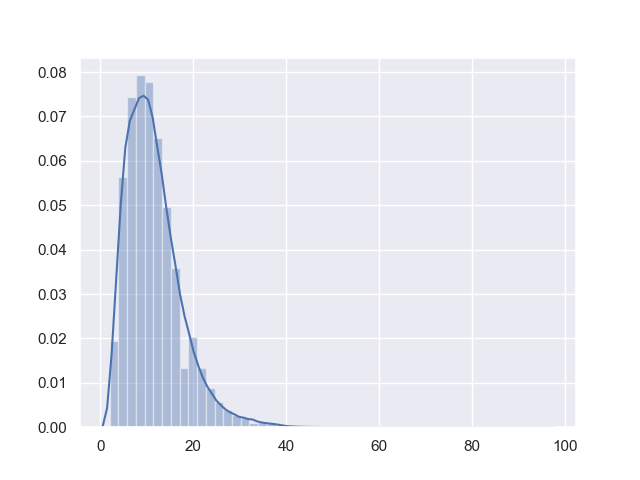
\includegraphics[width=0.5\textwidth]{images/title_lengths}
      \caption{Distribution of different title lengths}
\end{figure}\\
3. We convert the titles into array of integers, where each integer corresponds to the index of the word in the vocabulary list that we created, the index is between $1$ and $71057$, and we map all the special character that we added in step $2$ to $0$.\\
This vectorization process takes $\approx$ 2 hrs to run, therefore, we decide to store the vectorized data into a new .csv file, which we can use to train our data directly.

\section{References}
\noindent Convolutional Neural Networks for Sentence Classification By Yoon Kim\\
Judging a Book by its Cover By Brian et al.

\end{document}
